\chapter{Methodology}
This chapter includes different techniques to achieve tasks mentioned under objectives, in chapter one. This chapter describes how important sentences in a text document
can be identified. NGrams are discussed that can be used to identify key phrases in the text. Part of Speech Tagger (POS) assists in extracting Noun and Verb phrases
in the sentence. To determine whether a noun is a subject or an object, its ordinal position in the phrase and the type of sentence (whether active voice or passive
 voice) can 
be used. 

\section{Determining important sentences}
 For producing information rich extracts, \citeA{linOPP} described optimal position policy(OPP) emphasizing that sentence qualifying for extraction occur on different 
 ordinal position in text based on text genre and domain. 
\begin{itemize}
 \item Position hypothesis: Test Data including news articles and their summaries have been obtained from document understanding conference(DUC). This data can be processed
to discover if sentences included in summary follow a regular pattern, that is, important sentences have specific position in the source document. 
 \item Heuristics: Many heuristics have been adapted to generate summaries automatically. Taking first sentence of first paragraph, or first and last sentence from each paragraph
 has been a popular heuristic to generate summary. Such extraction methods have been part of early summarizer and have also been used as  baseline to evaluate summaries. 
\end{itemize}

Considering the popularity of Position Hypothesis, the test data(consisting of document, summary pairs) obtained from DUC is utilized. The test data contains news articles
and their summaries in separate files, both are tagged with document id for easy reference. Each sentence of the news article is assigned a number beginning with headline. 
The ordinal position of the sentences in the summary is then identified by comparing them against respective articles. 

Eight hundred ninety four (894) documents and summaries were processed for determining the which ordinal position of sentence is most frequent. Chart in figure 3.1 
shows the frequency distribution. 

\begin{figure}[h]
 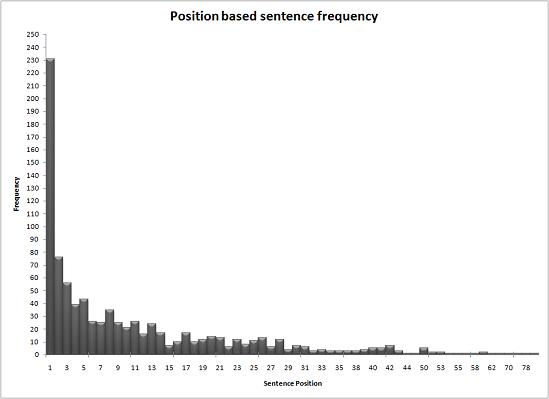
\includegraphics{/home/imran/Documents/myreport/Figure/sp2}
 \caption{\singlespace Frequency distribution shows 1st sentences is most frequent (231) times part of the summary}
 \label{ch3:sp2}
\end{figure}

\begin{figure}[h]
 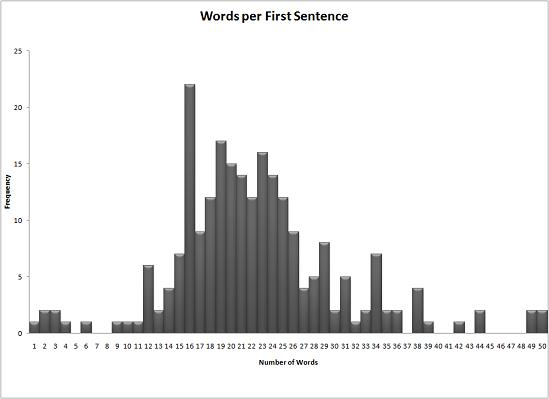
\includegraphics{/home/imran/Documents/myreport/Figure/sp4}
 \caption{\singlespace Number of words per first sentence}
\end{figure}

The chart shows that the first few sentences (1 to 5) are frequently extracted as summary, also the spikes of the bar chart lower down to zero as ordinal position increases.
The graph clearly indicates that information rich contents are clustered in first paragraph. Another interesting analysis is that of number of words contained in the first 
sentence. The chart in figure 3.2 is constructed by considering 1st sentence word counts. 

It can be noticed from the chart that the average word count is between 15 to 20, 22 to be more exact. Since the task of encapsulation requires a single best sentence
that can be further compressed to subject, verb, object, some mechanism of ranking sentences should exist that can assist in selecting best sentence suitable 
for encapsulation.
\section{n-grams}
``An n-gram is a subsequence of n items from a given sequence'' \citeA{webwikingram}. Items in this definition can refer to syllables, letters or words. Some examples of word level bigrams are: 
Knowledge base, Information Management, and Application Software. ``Google uses n-gram models for a variety of R\&D projects, such as statistical machine translation, 
speech recognition, checking spelling, entity recognition, and data mining. In September 2006 Google announced that they made their n-grams public at the Linguistic 
Data Consortium (LDC)''. Words that are parts of bigrams that repeat more than once in text are good terms to describe the text's contents; this is concluded
by \citeA{Ledeneval-FreqSequences}. We can use n-grams to extract sentences, ranking higher those sentences, which contain more n-grams. N-grams can also be used 
to re-rank sentences after extraction has been performed using position hypothesis. Since n-grams operate on a narrower unit of text that is
phrases or words, they are very useful in pointing out important portions of sentence which is desirable for sentence compaction.
\section{POS Tagger}
``In corpus linguistics, part-of-speech tagging (POS tagging or POST), also called grammatical tagging or word-category disambiguation, is the process of marking up the
words in a text (corpus) as corresponding to a particular part of speech, based on both its definition, as well as its context —i.e. relationship with adjacent and 
related words in a phrase, sentence, or paragraph'' \citeA{webwikipos}. In order to produce a good summary, it is essential to parse text and uncover the linguistic features.
Although parsing text is not termed as a robust technique for a voluminous corpus, it is suitable for processing comparatively small size document such as news articles. 


\clearpage
   
 